\section{边值问题}
\label{sec:ellip-bvp}

一根细棒两端浸在冰水里，棒内各处均匀发热。温度稳定之后是什么样子？棒上任何一小段都处在收支平衡中：流进来的热量加上这一段自己产生的热量，等于流出去的热量。这个平衡关系就是方程的来源。

\paragraph{区间上的平衡}
设棒占据区间$(0,1)$，$u(x)$是稳定后的温度，$f(x)$是单位长度上的发热率，$q(x)$是$x$处向右流过的热流。取一小段$[x,x+\delta]$，如图~\ref{fig:ellip-flux-balance}(a)。稳态时这一段的热量不变，流出减流入等于内部产热：
\[
 q(x+\delta)-q(x)=\int_x^{x+\delta}f(s)\,\mathrm{d}s .
\]

两边除以$\delta$，令$\delta\to0$，得到$q'=f$。再用导热定律把热流与温度联系起来：热量从高温流向低温，流量正比于温度梯度，比例系数$a(x)>0$是导热率，即$q=-a\,u'$。代入后得到
\begin{equation}
 -\bigl(a(x)\,u'(x)\bigr)'=f(x),\qquad x\in(0,1).
 \label{eq:ellip-1d-equation}
\end{equation}

\begin{BookInlineFigure}
  \centering
  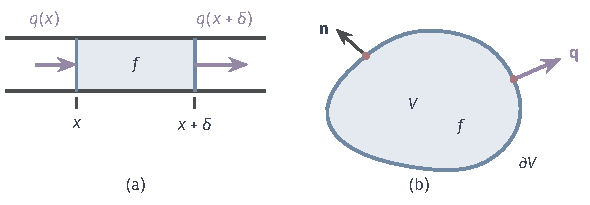
\includegraphics[width=100mm]{figures/06-differential-equations/02-partial-differential-equations/tikz/ellip-flux-balance/figure.pdf}
  \caption{热量收支平衡。(a)区间上的一小段：从左端流入$q(x)$，从右端流出$q(x+\delta)$，两者之差由段内的源项$f$补足。(b)多维区域中的控制体$V$：紫色箭头是热流$\bm{q}$，黑色箭头是边界的外法向$\bm{n}$，穿过$\partial V$的净流出量等于$V$内的总产热。}
  \label{fig:ellip-flux-balance}
\end{BookInlineFigure}

式~\eqref{eq:ellip-1d-equation}是二阶常微分方程，但它的提法与第~\ref{chap:ordinary-differential-equations}章的初值问题不同。初值问题在同一点给出$u$和$u'$，解可以从左向右递推。这里的两个条件分别放在区间的两端，右端的温度会影响左端，无法从一头推到另一头，必须把整段一起解出来。

取$a=1$、$f=1$，两端温度为零。方程$-u''=1$的解是
\begin{equation}
 u(x)=\frac{x(1-x)}{2},
 \label{eq:ellip-running-solution}
\end{equation}
它在中点取最大值$u(1/2)=1/8$。这个例子贯穿全章。后面每种方法算出的结果，都可以拿它来核对。

\paragraph{多维的散度型方程}
把收支平衡搬到区域$\Omega\subset\mathbb{R}^{d}$上。热流现在是向量场$\bm{q}(\bm{x})$，任取控制体$V\subset\Omega$，如图~\ref{fig:ellip-flux-balance}(b)，净流出量等于总产热：
\[
 \int_{\partial V}\bm{q}\cdot\bm{n}\,\mathrm{d}S=\int_Vf\,\mathrm{d}\bm{x} .
\]

由散度定理（可参考\BookChapterRef{chap:integral-theorems}{卷二第27章“积分定理”}），左端等于$\int_V\nabla\cdot\bm{q}\,\mathrm{d}\bm{x}$。这个等式对每个小控制体都成立，被积函数连续时可得$\nabla\cdot\bm{q}=f$。

导热率在不同方向上可能不同，例如木材顺纹与横纹导热差别很大，所以导热定律写成$\bm{q}=-\bm{A}(\bm{x})\nabla u$，其中$\bm{A}(\bm{x})$是$d\times d$的\term{扩散系数矩阵}（diffusion coefficient matrix）。于是得到散度型方程
\begin{equation}
 -\nabla\cdot\bigl(\bm{A}(\bm{x})\nabla u\bigr)=f\qquad\text{于}\ \Omega.
 \label{eq:ellip-divergence-form}
\end{equation}

取$\bm{A}=\bm{I}$，方程化为\term{Poisson方程}（Poisson equation）
\begin{equation}
 -\Delta u=f\qquad\text{于}\ \Omega,
 \label{eq:ellip-poisson}
\end{equation}
其中$\Delta u=\sum_{i=1}^d\partial_{i}^2u$是Laplace算子。$f=0$时称为Laplace方程，它的解称为\term{调和函数}（harmonic function）。方程前面的负号让$f>0$对应发热：$-\Delta u>0$表示$u$在该点附近比周围的平均值高，这正是热源处温度的样子。

第~\ref{chap:pde-problems}章按二阶项系数的符号结构区分方程类型：系数矩阵对称正定是椭圆型，还有一个时间方向上的一阶导数是抛物型，时间与空间的二阶导数异号是双曲型。式~\eqref{eq:ellip-divergence-form}没有时间，$\bm{A}$正定，就是椭圆型的典型代表。

\paragraph{三类边界条件}
方程只说明区域内部的收支，边界上发生什么要另外指定。设$\Omega$有界，$\bm{n}$是$\partial\Omega$上的外法向，$g$是边界上给定的函数。常用的条件有三类：

\begin{itemize}
 \item \term{Dirichlet边界条件}（Dirichlet boundary condition）$u=g$：边界温度由外界固定，如贴在恒温槽上。
 \item \term{Neumann边界条件}（Neumann boundary condition）$\bm{n}\cdot\bm{A}\nabla u=g$：规定穿过边界流入的热流。由$\bm{q}=-\bm{A}\nabla u$，$-\bm{q}\cdot\bm{n}$是单位面积上的流入量，$g=0$表示绝热。
 \item \term{Robin边界条件}（Robin boundary condition）$\bm{n}\cdot\bm{A}\nabla u+\beta u=g$，其中$\beta\geq0$：通过边界与环境换热，换热量正比于边界温度与环境温度之差，$g/\beta$相当于环境温度。
\end{itemize}

三者也可以分片出现在边界的不同部分。图~\ref{fig:ellip-boundary-types}固定源项$f=1$和左端$u(0)=0$，只改变右端的条件。绝热端把所有热量都存在棒内，温度最高；固定温度的右端可以直接散热，温度最低；Robin条件介于两者之间。

\begin{BookInlineFigure}
  \centering
  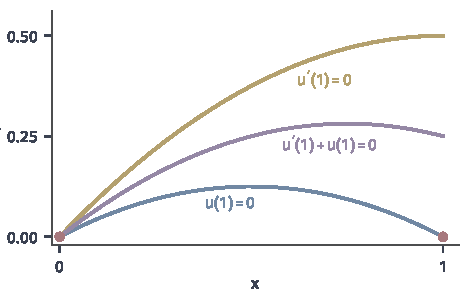
\includegraphics[width=80mm]{figures/06-differential-equations/02-partial-differential-equations/matplotlib/ellip-boundary-types/figure.pdf}
  \caption{同一方程$-u''=1$、同一左端条件$u(0)=0$，右端换三种条件。蓝线$u(1)=0$，解为$x(1-x)/2$；紫线$u'(1)+u(1)=0$，解为$3x/4-x^2/2$；黄线$u'(1)=0$，解为$x-x^2/2$。红点标出取定的边界值。}
  \label{fig:ellip-boundary-types}
\end{BookInlineFigure}

这三个解都可以手算验证。三者都有$-u''=1$和$u(0)=0$，因而都形如$u=Bx-x^2/2$，右端的条件只决定常数$B$：$u(1)=0$给出$B=1/2$，$u'(1)=0$给出$B=1$，$u'(1)+u(1)=0$即$(B-1)+(B-\tfrac12)=0$，给出$B=3/4$。

\paragraph{一致椭圆系数}
后面所有定理都要用到$\bm{A}$的一条性质。在式~\eqref{eq:ellip-divergence-form}两边乘以$u$并积分，会出现二次量$\int\nabla u^\top\bm{A}\nabla u$，它衡量的是梯度带来的能量。我们要求这个量能够控制梯度本身的大小，并且系数不能大到无界。

\begin{definition}[一致椭圆]
\label{def:ellip-uniform}
设$\bm{A}:\Omega\to\mathbb{R}^{d\times d}$可测。若存在常数$0<\kappa_{\min}\leq\kappa_{\max}<\infty$，使几乎所有$\bm{x}\in\Omega$和所有$\bm{\xi}\in\mathbb{R}^{d}$满足
\begin{equation}
 \bm{\xi}^\top\bm{A}(\bm{x})\bm{\xi}\geq\kappa_{\min}\lVert\bm{\xi}\rVert_2^2,\qquad
 \lVert\bm{A}(\bm{x})\bm{\xi}\rVert_2\leq\kappa_{\max}\lVert\bm{\xi}\rVert_2,
 \label{eq:ellip-uniform}
\end{equation}
就称$\bm{A}$在$\Omega$上\term{一致椭圆}（uniformly elliptic）。
\end{definition}

定义不要求$\bm{A}$连续，也不要求对称。系数可以在两种材料的交界处跳变，这在应用中很常见。若$\bm{A}$对称，第一个条件说$\bm{A}(\bm{x})$的最小特征值不小于$\kappa_{\min}$，第二个条件说最大特征值不超过$\kappa_{\max}$。

对任意足够光滑的$u$，取$\bm{\xi}=\nabla u(\bm{x})$，再对$\bm{x}$积分，得到
\begin{equation}
 \int_\Omega\nabla u^\top\bm{A}\nabla u\,\mathrm{d}\bm{x}\geq\kappa_{\min}\int_\Omega\lVert\nabla u\rVert_2^2\,\mathrm{d}\bm{x}.
 \label{eq:ellip-gradient-control}
\end{equation}
这就是一致椭圆的用途：无论梯度指向哪个方向，都有不低于$\kappa_{\min}$的“导热能力”把它计入能量。

图~\ref{fig:ellip-ellipticity}用集合$\{\bm{\xi}:\bm{\xi}^\top\bm{A}\bm{\xi}=1\}$的形状区分三种情况。(a)中$\bm{A}$的元素是$2,0.6,0.6,1$，特征值约为$2.28$和$0.72$，水平集是夹在两个圆之间的椭圆，这是椭圆一词的来历。

(b)中$\bm{A}=\operatorname{diag}(1,0)$，$\xi_2$方向的梯度完全不被计入，能量控制不住这个方向，方程在$x_2$方向没有扩散，这是退化情形。(c)中$\bm{A}=\operatorname{diag}(1,-1)$不定，水平集是双曲线，二次量可以取负，这是波动方程的结构，第~\ref{chap:wave-equations}章要用完全不同的方法处理。

\begin{BookInlineFigure}
  \centering
  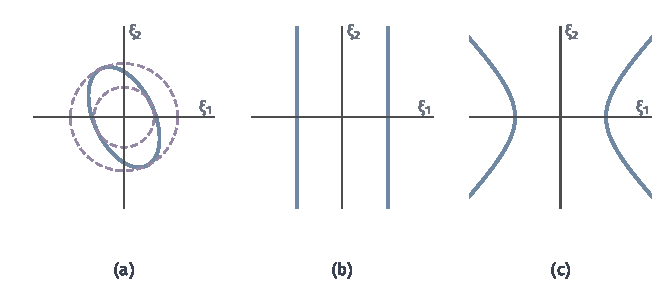
\includegraphics[width=112mm]{figures/06-differential-equations/02-partial-differential-equations/matplotlib/ellip-ellipticity/figure.pdf}
  \caption{水平集$\bm{\xi}^\top\bm{A}\bm{\xi}=1$（蓝线）的三种形状。(a)一致椭圆：椭圆被夹在半径$\kappa_{\max}^{-1/2}$与$\kappa_{\min}^{-1/2}$的两个圆（紫色虚线）之间。(b)退化：$\bm{A}=\operatorname{diag}(1,0)$，水平集是两条平行线，$\xi_2$方向无界。(c)不定：$\bm{A}=\operatorname{diag}(1,-1)$，水平集是双曲线。}
  \label{fig:ellip-ellipticity}
\end{BookInlineFigure}

要注意，主部一致椭圆只说明最高阶项的结构。方程$-\Delta u-k^2u=f$的二阶项与Poisson方程相同，零阶项的符号却相反，它在某些$k$上会失去唯一性，后面的结论不能照搬。本章的主线是式~\eqref{eq:ellip-divergence-form}，低阶项在用到时单独说明条件。
